\chapter{Käytännön esimerkki\label{example}}

Tutkielmassa on nyt käsitelty DevOps-toimintallia ja sen yhteydessä käytettäviä julkaisutapoja ja orkestrointiratkaisuja.
Helsingin Yliopiston Norppa-palautejärjestelmän kehitys perustuu DevOps-toimintamalliin ja käyttää monia tutkielmassa käsiteltyjä teknologioita.
Palvelun perustoiminta ja ohjelmistoarkitehtuuri esitellään osana tutkielmaa.


\section{Norppa-palautejäjestelmä}

Helsingin yliopiston tietojenkäsittelytieteen osaston sovelluskehitysakatemian (\textit{Toska}) \cite{Tenhunen23} kehittämä kurssipalautejärjestelmä Norppa on tutkielmassa esitetyn DevOps-toimintamallin mukaisessa aktiivisessa kehityksessä.
Järjestelmää käytetään Helsingin Yliopiston lisäksi myös Tampereen yliopiston kurssipalautejärjestelmänä \cite{Tampere23}.

Norppa on integroity Sisu-opintotietojärjestelmän kanssa. Järjestelmä luo automaattisesti palautelomakkeen ja tiedottaa Sisussa luodun kurssin opiskelijoille palautteesta.
Annetusta palautteesta luodaan yhteenveto, joka näytetään kurssin opiskelijoille ja opettajille.
Norppa tukee myös mmun muassa avointa tekstuaalista jatkuvaa palautetta ja koulutusohjelma- sekä yliopistotason palautteen yhteenvetonäkymiä.

Järjestelmän on kehittänyt Helsingin Yliopiston Toska-tiimi, mutta jatkokehitystä tehdään yhteistyössä Tampereen yliopiston kanssa.
Kehitys perustuu avoimeen lähdekoodin ja DevOps-toimintamalliin.
Seuraavaksi esitellään Norpassa käytetyt tutkielman kannalta merkitykselliset tekniset ratkaisut.

\section{Käytetyt ratkaisut}



\begin{figure}[ht]
\begin{center}
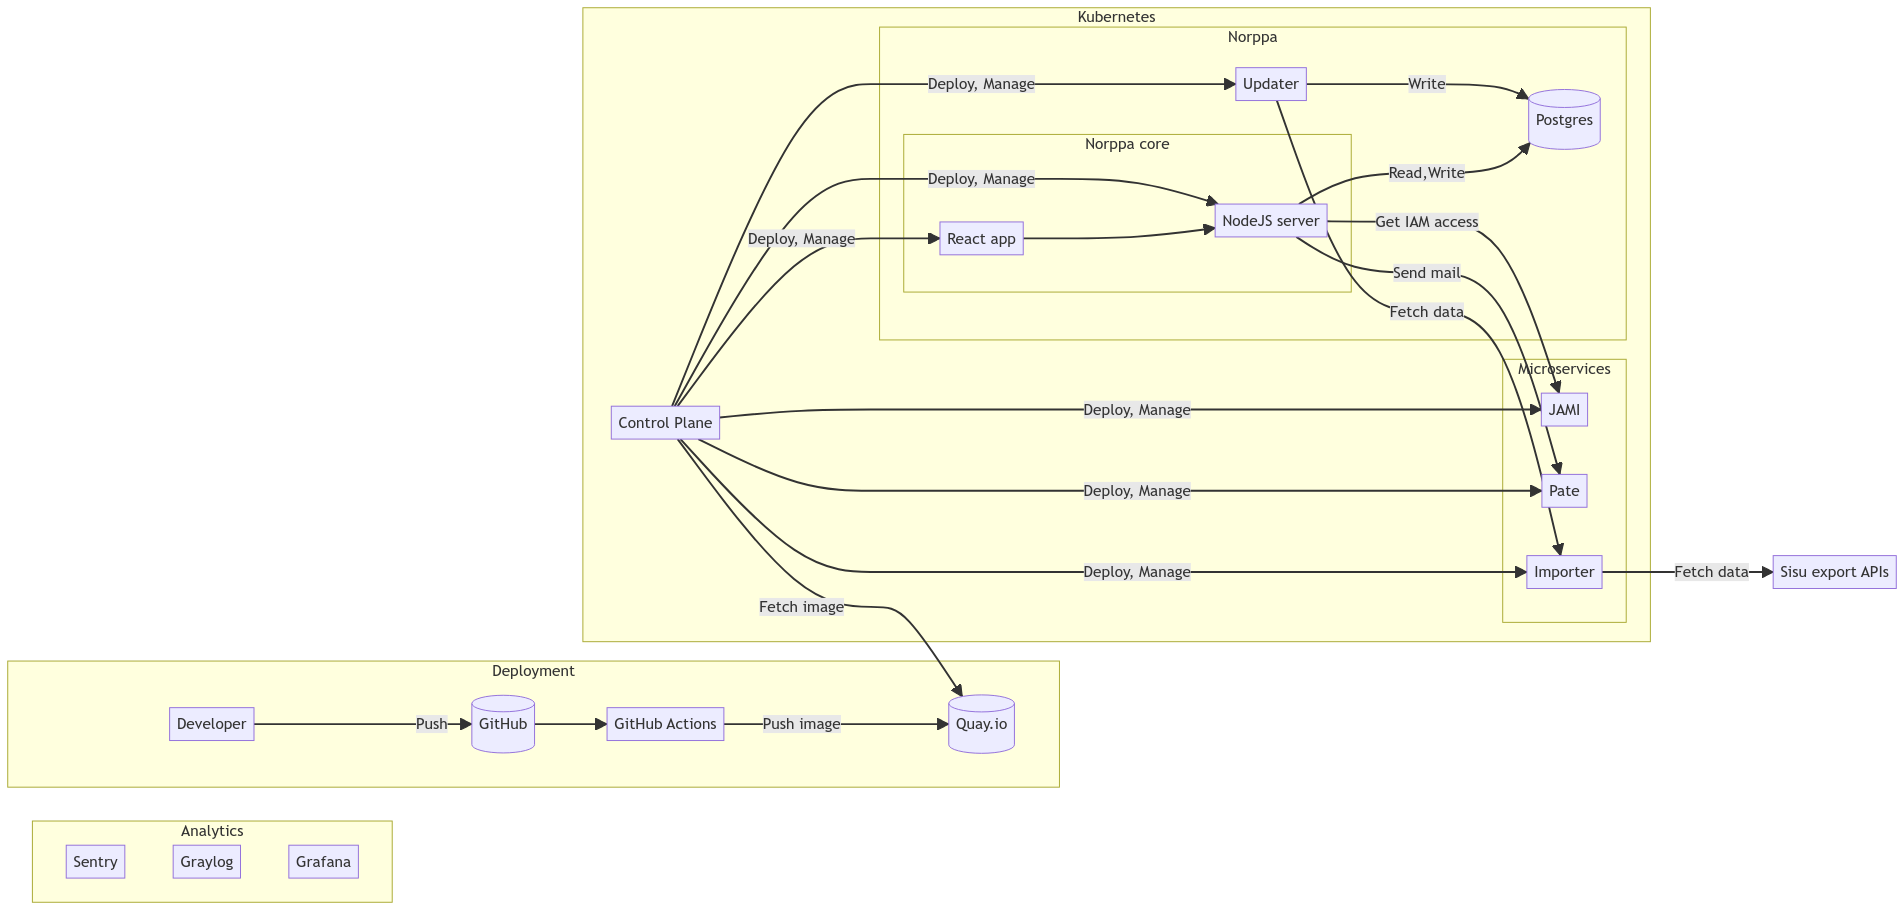
\includegraphics[width=1\textwidth]{figures/norppa_diagram.png}
\caption{Norppa-palautejärjestelmän laajennettu julkaisu- ja arkkitehtuuridiagrammi \cite{Norppa23}\label{fig:norppa}.}
\end{center}
\end{figure}
